\documentclass[12pt]{article}
 
\author{
        Troels, Troels, Kasper
}
\date{\today}

\usepackage{graphicx}
 
\title{Design}
 
\begin{document}
 
\maketitle

\section{Problem analysis}

Our design constraints are heavily influenced by the very specific use
case outlined in the problem assignment.  For clarity, we shall
outline the assumptions on which we have created our design.

\begin{description}
\item[Malcolm is a novice user,] and he will likely not understand
  complex versioning operations like branching or tagging.
  Additionally, he is the only one using the system: there is no need
  for a notion of multi-user support, or synchronisation against a
  remote/central repository.
\item[The versioning system is for documents,] not arbitrary files
  managed by the operating system (such as logs, for example).  This
  also implies that performance is not a chief concern.
\item[The central purpose is preventing data loss,] so it is more
  important to ensure that older versions can be restored than to
  provide advanced facilities for inspecting the history of a file.
  The ability to inspect a log of changes to a file is only important
  insofar as it helps the user find the last revision containing his
  missing data.
\item[Portability is somewhat of a concern,] as the assignment
  mandates we use FUSE, ostensibly for reasons of portability.
\item[The system has to be transparent,] and we cannot ask Malcolm to
  alter his usual work routine in any way.  When he clicks the
  \texttt{Save}-button in his program, we have to make sure older
  revisions of the working document are not lost.
\end{description}

\section{Design requirements}

Our implementation must make use of FUSE; this is an external
requirement mandated by the course.  However, FUSE is not a bad
choice: the purpose of our file system is not to store versioned data
efficiently on a physical disk; thus we do not need direct access to
hardware devices, and it is therefore not necessary for our file
system to run in kernel mode.  Running a file system in user space
drastically lowers the risk of major system crashes, as it will be as
limited as any ordinary process\cite{EGGERT:1993mz}.  FUSE provides an
effective and simple way to provide a completely transparent file
system interface, and makes it somewhat easy to use a standard native
file system for the actual data storage.  On the downside, should the
needs of our system evolve in the future, to the point where
performance and efficient storage becomes of paramount concern, it may
be hard to achieve such results outside of kernel mode.  However, as
stated in the textbook, such a radical change in functional
requirements merits an entirely new design and implementation, not an
upgrade of an existing one.

The versioning must be completely transparent to the user, who must be
able to work in complete ignorance of the fact that previous
iterations of his work is being safely stored.  For each file, a
linear history of revisions will be stored.  Directories will not be
versioned, only their contents.  Symbolic and hard links will
\textit{not} be supported: a novice user will not make use of these
facilities in any case, and they create enormous complexity, far
beyond any potential utility, given our usage scenario.

The goal is to create one new revision per ``save'' in the users
application.  This follows the design principle of doing what is most
obvious to a user.  FUSE (or most common file system interfaces, for
that matter) does not explicitly describe such an operation.  Hence,
some other heuristic will have to be specified to determine when to
store a new revision of a file.

Unless access is done through special mechanisms, only the
\textit{most recent} version of a file should be visible and
accessible.  For example, if a file has been deleted, it must not show
up in directory listings.  This ensures compatibility with existing
programs that interact with files (such as search programs, which
should not find deleted files or earlier revisions).

There must be some way of accessing the revision history in a purely
\textit{read-only} manner in order to restore old revisions.  It must
not be possible to modify the revision history through our provided
interfaces.
 
\section{Choice of Language}
 
A fundamental, and early, design choice is selection of implementationlanguage. Our choice is constrained by several factors, in roughly
descending order of priority:
 
\begin{description}
\item[Existing familiarity: ] We have a hard deadline on
  implementing the design, and the allotted period of time is not
  particularly long. Notably, we do not have a significant amount of
time to invest in learning new languages, so we must all be somewhat  familiar with the language, or at least able to swiftly pick up the
  necessary knowledge.
\item[Availability of FUSE bindings: ] No matter the language, we will  most likely not have time to develop (and debug) a new set of
  bindings to FUSE. The language we choose must thus have an existing
  (mature) binding.
\item[Development efficiency: ] As mentioned above, we do not have a
  lot of time to write the code, so the language choice should be
  optimised for developer productivity over such things as final
  program performance.
\item[Implementation portability: ] According to the assignment,
  portability to OS X and GNU/Linux is a goal. Hence, our chosen
  language must have somewhat mature implementations on both of these
  systems.
\item[Safety: ] A filesystem is a central and important construction,
  and it is important that it is reliable and correct. We will likely
  not have time to do heavy testing of our work, and it is therefore
  desirable that our chosen language provides as many static
  guarantees of correctness as possible.
\end{description}
 
Based on these parameters, we have chosen Python. We are all somewhat
familiar with the language, and we have faith in the maturity of its
FUSE bindings due to the explicit recommendation of Python by the
course lecturers. Python is also generally acknowledged as a
productive language, and the reference implementation (CPython) is
ported to all relevant platforms. Python does suffer a bit in the
area of static safety guarantees, though arguably less so than C
(another obvious possibility), but significantly more than languages
such as Haskell or OCaml.
 
We assume that the possibility of using the Bourne shell scripting
language is a somewhat morbid joke.
 
\section{Storage backend}

Irrespective of the external interface of our file system, we have to
design a backend that can store earlier (and current) versions of
files.

The file system we are supposed to end up with should only support a
single user.  The primary goal is to allow the user to go back to an
earlier version of any file. It's not suggested that the user should
have several different current versions of the same file (no
branching).

By using these specifications we have to decide whether to implement
our own version control or use an existing such as Subversion or
Git\cite{Grant:2009ly}.

Using an already existing version control system we not have to
implement any actual data-compression or logic for handling revisions.
Instead we would have to create an interface for the chosen version
control system. This seems to be the easier choice, but we think the
version control systems that exist are too complex for the simple
needs of this file system. Implementing our own system has the
advantage of not adding more complexity than needed.

Branches aren't needed as the user is not supposed to have multiple
versions of the same file active. Therefore merges aren't needed.
There is no need for collaboration either. All in all Git and
Subversion, which are the two version control systems we considered,
are too complex, so we decided to implement our own simple system.

Our system (as is not unusual in FUSE) is based on the notion of a
\textit{stacked} file system, which functions as a layer, or wrapper,
around a traditional, physical on-disk filesystem.  This design, and
terminology, is presented in \cite{1096690}, which notes greatly
improved implementation simplicity over a classic physical filesystem
implementation, as well as a negligible performance impact.  The use
of a stacked file system is also mentioned in
\cite{Bustamante04wayback:a}.

In summary, our system will work by storing version data in the form
of normal files on a traditional file system, and using this data to
translate FUSE operations into operations on this versioning data.
 
\section{Feeing up disk space}

To be able to go back to old versions of files we would have to keep
all the old data stored somewhere. After some time most of the disk
space would be filled with old versions of files. This can be
postponed by only recording changes to files, but it would still
happen. Some mechanism to clean out old, unused versions of files must
therefore be implemented.

We have decided that implementing a cleaner-process as discussed in
\cite{319159} would be the right solution. As the assignment states that
the file system should only be used in the Documents directory, we
assume that all the files are actually user-created files. We also
assume that all files in the directory are equally important to keep
old revisions of. This allows us to use a simpler policy than
described in the article. Instead of having different policies for
different groups of files we are able to have a global policy for the
entire file system.

\subsection{File retention policies}
We have decided to use a policy that use a mixture of two different
policies, based on time of the revision. If a revision is less than
one month old the Keep All-policy is used. This saves all changes to
the file, which takes up the most space. When a revision is older than
one month the policy changes to Keep Landmarks, which means that
revisions close to each other, time wise are deleted except the
newest. This is useful as the older revisions get the less likely the
user is to know the difference between two adjacent revisions, and the
eldest revision is the most likely to be unneeded.
The one-month limit and the decision about when two files are close to
each other should be changeable by the user, as the need for cleanup
is based on several things such as disk size, importance of files etc.

\subsection{File-locking}
This process has to be able run concurrently with the file system
being in use. The worst case scenario being that a user is trying to
retrieve a version of a file while the cleaner-process deletes it. To
avoid this, the file system and the cleaner-process has to have a way
to tell each other when a file is in use. We have decided to implement
this using the rename system call, as it is promised to be atomic. In
the version-folder for a given file an .unlocked-file is located.
Whenever either the cleaner-process or the file system wants to use
the file, they have to rename .unlock to .lock. This guarantees that
if the rename-call is successful, it is the only process accessing the
file at a given time. If the other process tries to access the same
file it will have to wait until the file is renamed back to unlock
again.

\subsection{Locating files to check}
As the number of files grows a way to identify files likely to be
ready for cleanup is needed. When there is only a small amount of
files the cleaner-process can just check all of them at every
iteration, but as soon as the number of files grow it becomes
unfeasible. A way to identify files that are likely to have revisions
that can be deleted is therefore needed.

To avoid having to scan the file system for files a list of all the
files on the system should be kept in memory. Together with each entry
in the list a date is kept that signify when the cleaner-process
should analyze the file again. This is a simpler implementation of the
way it is done in the Elephant file system \cite{Santry:1999gf}. When
the cleaner-process has analyzed the file a new date is created
according to the findings. The exact intervals at which files should
be analyzed has to be worked out during testing.

\section{File system interface}
A somewhat small decision when designing with enormous impact for the
user is the way that files are shown to the user.
We have to decide on how the user sees the different versions of the
file. A possibility is to show all available versions of all the
files,
which has the advantage that the user can easily see every single
change to all files, but this quickly becomes a problem.
As soon as there are more than a few files or versions it becomes
impossible to get an overview of the files in a directory.
Instead we have decided that it should be completely invisible to the
user that the file system is actually implementing version control.
This makes the file system usable by everybody and only if a user has
to get an earlier revision will he have to know the specifics about
the file system.

We have decided to expand the normal file system namespace to allow
the use of \texttt{<filename>;<version number>} to access older versions
of a file or \texttt{<directory>;*} to list all versions of the files
located in the directory. If the semicolon is omitted it assumes you
only wish to work with the most resent version.

Implementing access to the older versions trough the namespace also
have the huge advantage of allowing all existing programs that already
use the standard file system API to access the files directly without
the need of other tools.

\section{Internal file representation}
Since FUSE is located in user space, we use the native file system to
implement our own version control system. To meet the requirements of
the file system, it only needs to store different versions of the same
files. A files uniqueness is specified by its name in the name space
alone – meaning any new file named the same as some old deleted file
will obtain the history of the old file. The same is the case for
directories which in effect means no versioning of directories is
needed, only the need to be able to distinguish if a directory has
been deleted or not.

We can use that we have defined our name space to not accept suffixes
in the format of either \texttt{;<number>} or \texttt{;*} to allow direct access to
versioned files trough the name space with existing tools to help
represent the versioned files internally.

To represent the files we use the following rules:

\begin{itemize}
\item The name of any file in the system is given by a directory named
  \texttt{<filename>;0}. This directory contains files named by numbers that
  represent the version number of the file. The higher the number the
  newer the version.
\item If the file exist (not been deleted) a file with \texttt{<filename>} is
  located at the same level as the directory containing the
  versions. This file is always hard linked to the newest version
  located inside the files directory.
\item If the file is deleted the above mentioned file is removed and a
  new version is created by copying the latest. Should a new file be
  created with the same name a jump in version numbering will be
  created skipping one version as the new file is created. The reason
  for this is to be able to indicate that a file deletion has happened
  at the time of the last version before the jump in versions.
\item Renaming of a file means renaming both the hard link and the
  directory.
\item The name of any directory in the system is given by a directory
  named \texttt{<directory>;*}. All contents of the directory, such as files
  and subdirectories, is located inside this directory.
\item If the directory exist (not been deleted) a symbolic link is
  created named \texttt{<directory>} at the same level as the directory
  containing the contents. This symbolic link points to this
  directory.  Renaming of a directory means renaming both the symbolic
  link and the directory containing the contents of the folder.
\end{itemize}

It is worth noticing that renames happens directly on the
files/directories and is irrecoverable by means of our versioned file
system. An unresolved problem arise here since a rename to an already
used, but deleted, file or directory would not be allowed. This is not
possible to resolve using our current design, as we would require both
the history to follow a file trough renames to not loose history,
deleting the old files history would mean loss of history and a merge
of two versions would not make much sense. This would be confusing and
no good solution really exist for this problem no matter what system
is used. It would seem to the user as either the old or the new list
of old versions of the two files would seem to have disappeared or
multiple/merged lists would have to be displayed.

See figure \ref{structurefig}.

\begin{figure}
\begin{center}
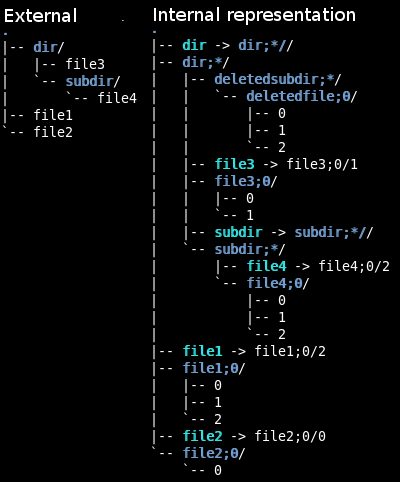
\includegraphics[height=150mm]{filestructure.png}
\end{center}
\caption{Example of logical versus physical file structure}
\label{structurefig}
\end{figure}

\section{Delta compression}

\section{Link-handling?}

\section{GUI interface?}


\bibliographystyle{abbrv}
\bibliography{assignment1}
 
\end{document}
 
